\begin{figure}[ht]
    \centering
    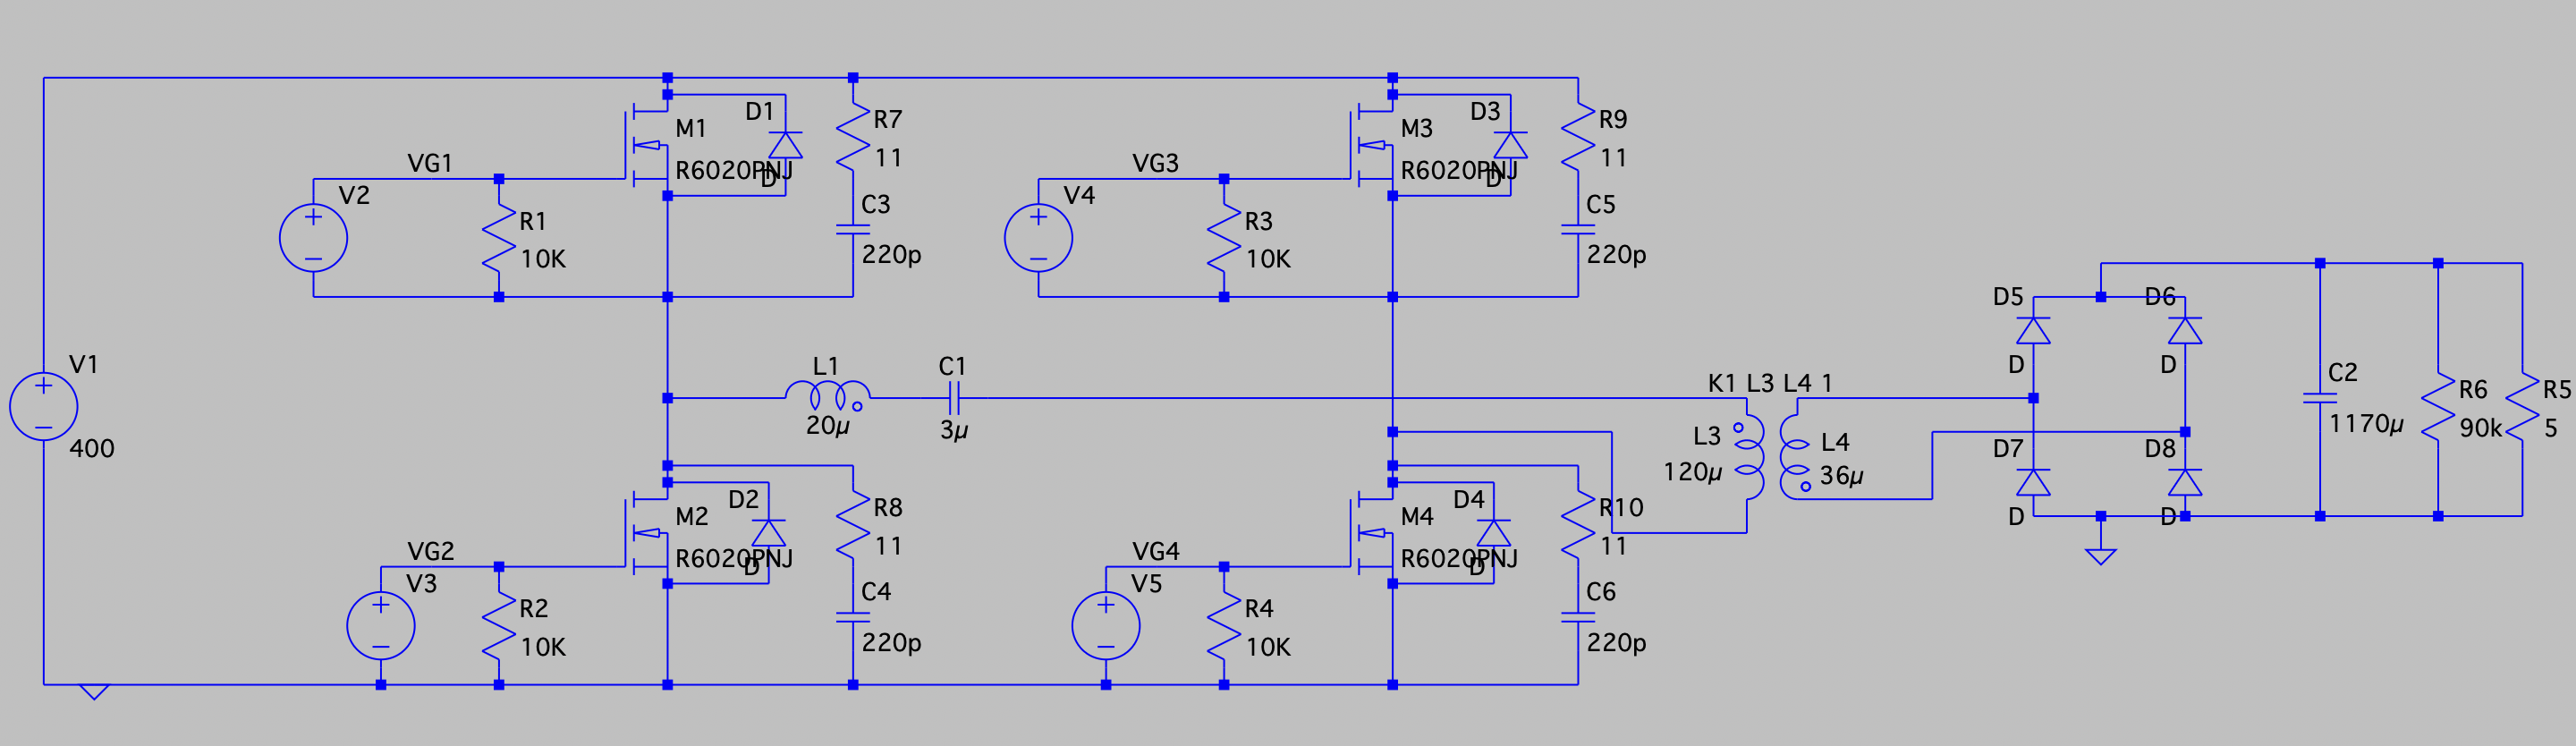
\includegraphics[width=\textwidth]{overall_circuit.png}
    \caption{Simulation}
    \label{fig:Simulation1}
\end{figure}

\subsection{Why Measure Phase Voltage?}


\begin{equation*}
    T_{line} =
    \begin{bmatrix}
        \frac{2}{3}  & \frac{1}{3}  & 0 \\
        \frac{-1}{3} & \frac{1}{3}  & 0 \\
        \frac{-1}{3} & \frac{-2}{3} & 0
    \end{bmatrix}
\end{equation*}



\subsection{Derivation of the Transformations}
For this conversion, we need to define a matrix, so let's look at the
derivation for such a matrix.

Let \( V_a, V_b, V_c \) be the phase voltages given by:
\[
    V_a = \sin(\omega t)
\]
\[
    V_b = \sin(\omega t - 120^\circ)
\]
\[
    V_c = \sin(\omega t + 120^\circ)
\]

The line voltages \( V_{ab}, V_{bc}, V_{ca} \) are given by:
\[
    V_{ab} = V_a - V_b
\]
\[
    V_{bc} = V_b - V_c
\]
\[
    V_{ca} = V_c - V_a
\]

Also, we know that:
\[
    V_a + V_b + V_c = 0
\]

Let us assume two matrices: \( P \), representing phase voltages, and \( L \),
representing line voltages:
\[
    P = \begin{bmatrix}
        V_a \\
        V_b \\
        V_c \\
    \end{bmatrix}
\]
\[
    L = \begin{bmatrix}
        V_{ab} \\
        V_{bc} \\
        V_{ca} \\
    \end{bmatrix}
\]

Let \( T \) be a transformation matrix from \( P \) to \( L \):
\[
    L = T \cdot P
\]

We can define \( T \) as:
\[
    T = \begin{bmatrix}
        1  & -1 & 0  \\
        0  & 1  & -1 \\
        -1 & 0  & 1  \\
    \end{bmatrix}
\]

Since the inverse of \( T \) does not exist, we redefine it as:
\[
    \begin{bmatrix}
        V_{ab} \\
        V_{bc} \\
        V_{ca} \\
        0      \\
    \end{bmatrix} = \begin{bmatrix}
        1  & -1 & 0  & 1 \\
        0  & 1  & -1 & 1 \\
        -1 & 0  & 1  & 1 \\
        1  & 1  & 1  & 1 \\
    \end{bmatrix} \begin{bmatrix}
        V_a \\
        V_b \\
        V_c \\
        0   \\
    \end{bmatrix}
\]

Taking the inverse of \( T \):
\[
    T^{-1} = \begin{bmatrix}
        \frac{2}{9}  & -\frac{1}{9} & -\frac{4}{9} & \frac{1}{3} \\
        -\frac{4}{9} & \frac{2}{9}  & -\frac{1}{9} & \frac{1}{3} \\
        -\frac{1}{9} & -\frac{4}{9} & \frac{2}{9}  & \frac{1}{3} \\
        \frac{1}{3}  & \frac{1}{3}  & \frac{1}{3}  & 0           \\
    \end{bmatrix}
\]

Solving the matrix:
\[
    V_a = \frac{2}{9}V_{ab} - \frac{1}{9}V_{bc} - \frac{4}{9}V_{ca}
\]
\[
    V_b = -\frac{4}{9}V_{ab} + \frac{2}{9}V_{bc} - \frac{1}{9}V_{ca}
\]
\[
    V_c = -\frac{1}{9}V_{ab} - \frac{4}{9}V_{bc} + \frac{2}{9}V_{ca}
\]

We also know that \( V_{ab} + V_{bc} + V_{ca} = 0 \), so:
\[
    V_{ca} = -V_{ab} - V_{bc}
\]

Thus:
\[
    V_a = \frac{2}{3}V_{ab} + \frac{1}{3}V_{bc}
\]
\[
    V_b = -\frac{1}{3}V_{ab} + \frac{1}{3}V_{bc}
\]
\[
    V_c = -\frac{1}{3}V_{ab} - \frac{2}{3}V_{bc}
\]

So, we can define the transformation matrix as:
\[
    T_{line}^{-1} = \begin{bmatrix}
        \frac{2}{9}  & -\frac{1}{9} & -\frac{4}{9} \\
        -\frac{4}{9} & \frac{2}{9}  & -\frac{1}{9} \\
        -\frac{1}{9} & -\frac{4}{9} & \frac{2}{9}  \\
    \end{bmatrix}
\]
